\section{MQ算术编解码器}
\subsection{编码器结构}
JPEG2000 所用的MQ 编码器结构如图{\ref{fig:mqStructure}}所示。输入由待编码位D和上下文矢量CX构成,输出为压缩之后生成的码流。\\
\indent MQ编码器是一种自适应二进制算术编码器。其中,自适应算术编码是指编码系统根据已经传输和编码的信息串,调整用来划分区间的当前符号概率估计。对于同一待编码位D,其上下文CX不同,则对应的符号概率并不一定相同。因此,必须读取CX当前状态的符号概率来确定消息的符号概率,同时决定是否要转移到下一状态。符号概率的状态转移表由标准提供,共47种状态。
\begin{figure}[H]
\centering  
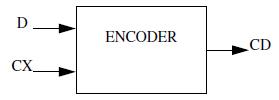
\includegraphics [scale=0.4]{mqStructure.jpg} 
\caption{MQ 编码器结构图} 
\label{fig:mqStructure} 
\end{figure}

\subsection{递归区间划分}
算术编码器按符号概率将符号分为大概率符号MPS和小概率符号LPS。如图{~\ref{fig:mpsLps}}所示,LPS区间在MPS区间之前。其中,A表示概率间隔长度,C表示概率间隔下限,则[C,C+A]即为编码区间。如果LPS 当前的概率估计值是Qe,编码当前符号后子区间的变化如下:\\
\indent\indent\indent 如果输入符号是MPS,$ A = A * (1 - Q_e), C = C + A * Q_e$\\
\indent\indent\indent 如果输入符号是LPS,$ A = A * Q_e, C $不变\\
\indent 由于乘法运算比较费时,为简化计算,可将区间A 保持在十进制[0.75,1.5]的范围内,此时A和C可近似为:\\
\indent\indent\indent 如果输入符号是MPS,$ A = A - Q_e, C = C + Q_e$\\
\indent\indent\indent 如果输入符号是LPS,$ A = Q_e, C $不变 \\
\indent 为了将A 保持在[0.75,1.5]的范围内,当整数值降到小于0.75 时,需通过重归一化把它加倍。重归一化发生时,调用概率估计模型,为当前正被编码的上下文确定一个新的概率估计。若将A 限制在十进制范围0.75-1.5 之间,概率区间的划分可以使用简单的算术近似方法。
\begin{figure}[H]
\centering  
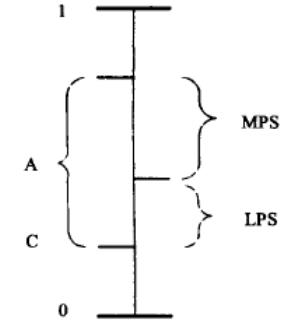
\includegraphics [width=2in]{mpsLps.jpg} 
\caption{MQ编码器编码区间示意图} 
\label{fig:mpsLps} 
\end{figure}

\subsection{编码流程}
首先对编码器进行初始化INTENC,然后读入上下文CX和待编字节D开始编码。编码时判断D是大概率符号还是小概率符号。如为大概率符号,进行CODEMPS编码;如为小概率符号,进行CODELPS编码。CODEMPS和CODELPS的编码流程如图{\ref{fig:codemps}}和图{\ref{fig:codelps}}所示。\textit{代码见函数entropy\_coding。}
\begin{figure}[H]
\centering  
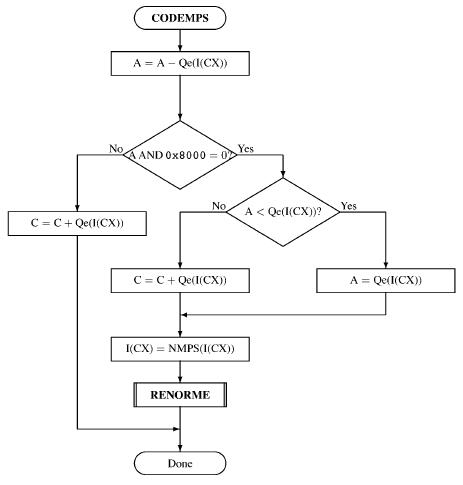
\includegraphics [width=3.5in]{codemps.jpg} 
\caption{CODEMPS流程图} 
\label{fig:codemps} 
\end{figure}

\begin{figure}[H]
\centering  
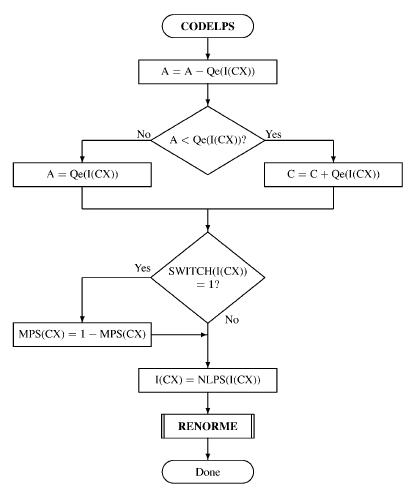
\includegraphics [width=3.5in]{codelps.jpg} 
\caption{CODELPS流程图} 
\label{fig:codelps} 
\end{figure}

\subsection{解码流程}
解码器根据CX和CD,一次解码一个二进制数据(如图{\ref{fig:mqDeStructure}}所示)。同编码时一样,在解码工程中,同步调整用来划分区间的当前符号概率估计。\textit{代码见函数entropy\_decoding。}
\begin{figure}[H]
\centering  
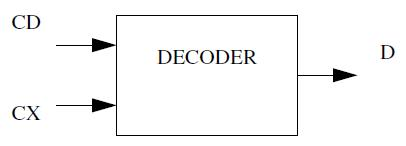
\includegraphics [width=2in]{mqDeStructure.jpg} 
\caption{MQ 解码器结构图} 
\label{fig:mqDeStructure} 
\end{figure}